\begin{frame}[fragile]
  \begin{center}
    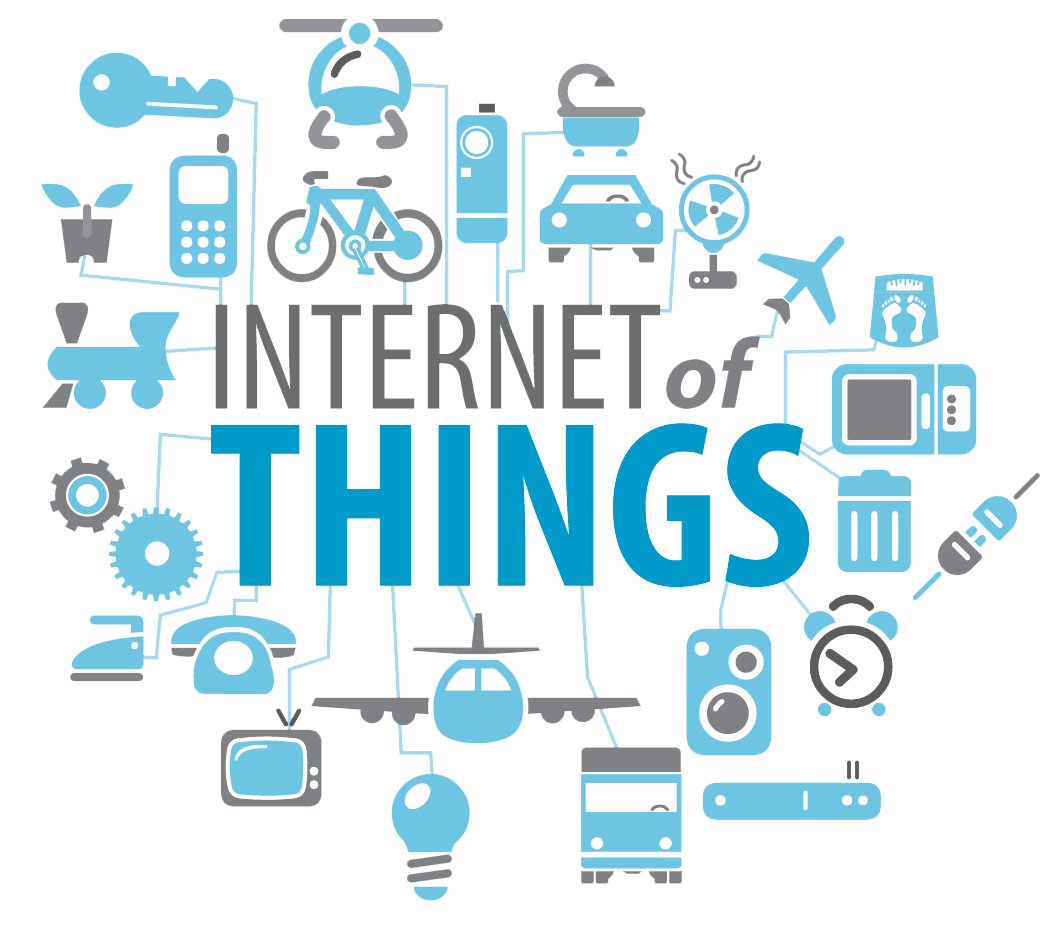
\includegraphics[width=0.9\textwidth]{images/iot}
    \label{fig:iot}
  \end{center}
\end{frame}

\begin{frame}{Internet of Things}
  \Large
  \begin{itemize}
    \item Alltägliche Geräte
    \item Zugang zu IP-Netz
    \item Unterstützung des Menschen
  \end{itemize}

  \vspace{0.5cm}

  \begin{quote}
    \normalsize
    Das Ziel des \textbf{Internets der Dinge} ist es, die Informationslücke
    zwischen der realen und virtuellen Welt zu minimieren.
    \begin{flushright}
      \small
      -- Mattern, F. (2005), Das Internet der Dinge
    \end{flushright}
  \end{quote}
\end{frame}

\begin{frame}[fragile]
  \begin{center}
    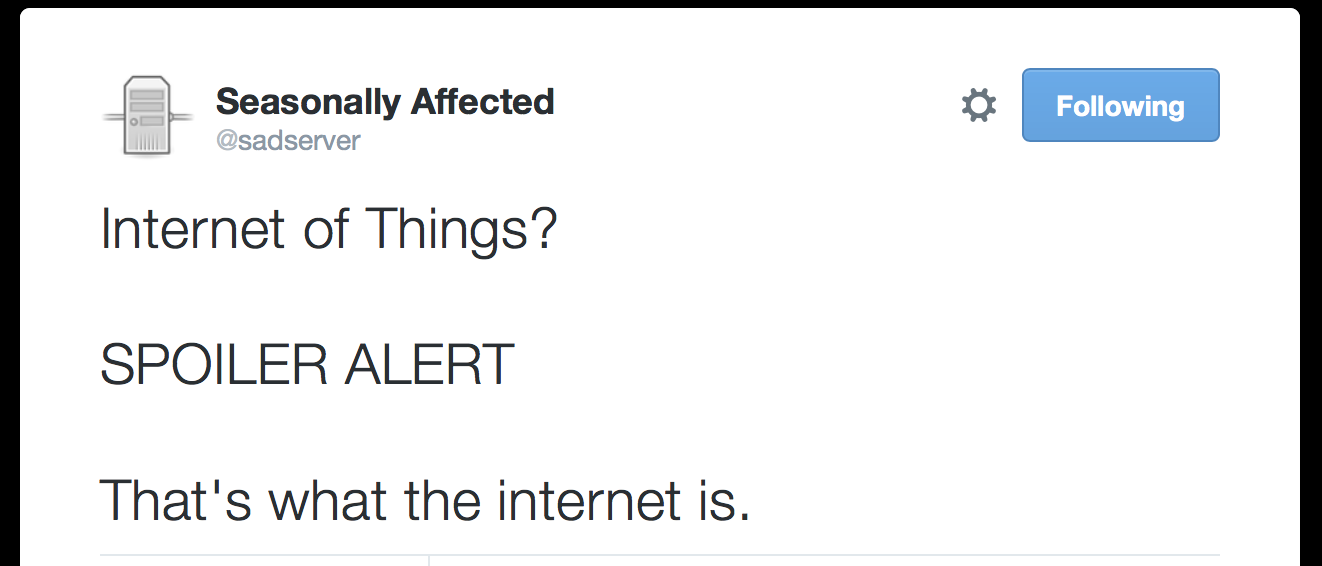
\includegraphics[width=0.75\textwidth]{images/sadserver1}
    \label{fig:spoiler}
  \end{center}
\end{frame}